\documentclass[a4paper,UKenglish,cleveref, autoref, thm-restate]{lipics-v2021}
%This is a template for producing LIPIcs articles. 
%See lipics-v2021-authors-guidelines.pdf for further information.
%for A4 paper format use option "a4paper", for US-letter use option "letterpaper"
%for british hyphenation rules use option "UKenglish", for american hyphenation rules use option "USenglish"
%for section-numbered lemmas etc., use "numberwithinsect"
%for enabling cleveref support, use "cleveref"
%for enabling autoref support, use "autoref"
%for anonymousing the authors (e.g. for double-blind review), add "anonymous"
%for enabling thm-restate support, use "thm-restate"
%for enabling a two-column layout for the author/affilation part (only applicable for > 6 authors), use "authorcolumns"
%for producing a PDF according the PDF/A standard, add "pdfa"

%\pdfoutput=1 %uncomment to ensure pdflatex processing (mandatatory e.g. to submit to arXiv)
%\hideLIPIcs  %uncomment to remove references to LIPIcs series (logo, DOI, ...), e.g. when preparing a pre-final version to be uploaded to arXiv or another public repository

%\graphicspath{{./graphics/}}%helpful if your graphic files are in another directory

\bibliographystyle{plainurl}% the mandatory bibstyle
%\title{On deadlock avoidance control for lock-sharing systems} 
\title{Broadcast networks with local registers}

%\titlerunning{Dummy short title} %TODO optional, please use if title is longer than one line

%\author{Jane {Open Access}}{Dummy University Computing Laboratory, [optional: Address], Country \and My second affiliation, Country \and \url{http://www.myhomepage.edu} }{johnqpublic@dummyuni.org}{https://orcid.org/0000-0002-1825-0097}{(Optional) author-specific funding acknowledgements}%TODO mandatory, please use full name; only 1 author per \author macro; first two parameters are mandatory, other parameters can be empty. Please provide at least the name of the affiliation and the country. The full address is optional. Use additional curly braces to indicate the correct name splitting when the last name consists of multiple name parts.

%\author{Joan R. Public\footnote{Optional footnote, e.g. to mark corresponding author}}{Department of Informatics, Dummy College, [optional: Address], Country}{joanrpublic@dummycollege.org}{[orcid]}{[funding]}

\author{Lucie Guillou}{IRIF, Université de Paris}{}{}{}
\author{Corto Mascle}{LaBRI, Université de Bordeaux}{}{}{}
\author{Nicolas Waldburger}{IRISA, Universit\'e de Rennes}{}{}{}

\authorrunning{L. Guillou, C. Mascle, N. Waldburger} %TODO mandatory. First: Use abbreviated first/middle names. Second (only in severe cases): Use first author plus 'et al.'

\Copyright{Lucie Guillou, Corto Mascle and Nicolas Waldburger} %TODO mandatory, please use full first names. LIPIcs license is "CC-BY";  http://creativecommons.org/licenses/by/3.0/

%\ccsdesc[100]{\textcolor{red}{Replace ccsdesc macro with valid one}}
%%TODO mandatory: Please choose ACM 2012 classifications from
%%https://dl.acm.org/ccs/ccs_flat.cfm

\begin{CCSXML}
	<ccs2012>
	<concept>
	<concept_id>10003752.10003753.10003761.10003763</concept_id>
	<concept_desc>Theory of computation~Distributed computing models</concept_desc>
	<concept_significance>500</concept_significance>
	</concept>
	</ccs2012>
\end{CCSXML}

\ccsdesc[500]{Theory of computation~Distributed computing models}

% \ccsdesc{Theory of computation~Models of computation~Concurrency~Distributed computing models}

\keywords{parameterized verification, concurrent systems, well quasi-orders} %TODO mandatory; please add comma-separated list of keywords



%\category{} %optional, e.g. invited paper

%\relatedversion{} %optional, e.g. full version hosted on arXiv, HAL, or other respository/website
%\relatedversiondetails[linktext={opt. text shown instead of the URL}, cite=DBLP:books/mk/GrayR93]{Classification (e.g. Full Version, Extended Version, Previous Version}{URL to related version} %linktext and cite are optional

%\supplement{}%optional, e.g. related research data, source code, ... hosted on a repository like zenodo, figshare, GitHub, ...
%\supplementdetails[linktext={opt. text shown instead of the URL}, cite=DBLP:books/mk/GrayR93, subcategory={Description, Subcategory}, swhid={Software Heritage Identifier}]{General Classification (e.g. Software, Dataset, Model, ...)}{URL to related version} %linktext, cite, and subcategory are optional

%\funding{(Optional) general funding statement \dots}%optional, to capture a funding statement, which applies to all authors. Please enter author specific funding statements as fifth argument of the \author macro.

%\acknowledgements{I want to thank \dots}%optional

%\nolinenumbers %uncomment to disable line numbering



%Editor-only macros:: begin (do not touch as author)%%%%%%%%%%%%%%%%%%%%%%%%%%%%%%%%%%
% \EventEditors{John Q. Open and Joan R. Access}
% \EventNoEds{2}
% \EventLongTitle{42nd Conference on Very Important Topics (CVIT 2016)}
% \EventShortTitle{CVIT 2016}
% \EventAcronym{CVIT}
% \EventYear{2016}
% \EventDate{December 24--27, 2016}
% \EventLocation{Little Whinging, United Kingdom}
% \EventLogo{}
% \SeriesVolume{42}
\ArticleNo{1}
%%%%%%%%%%%%%%%%%%%%%%%%%%%%%%%%%%%%%%%%%%%%%%%%%%%%%%




\newcommand{\cortoin}[1]{\todo[color=blue!20,inline]{\small #1}}
\newcommand{\corto}[1]{\todo[color=blue!20]{\small #1}}

\newcommand{\nicoin}[1]{\todo[color=red!20,inline]{\small #1}}
\newcommand{\nico}[1]{\todo[color=red!20]{\small #1}}

\newcommand{\luin}[1]{\todo[color=teal!20,inline]{\small #1}}
\newcommand{\lu}[1]{\todo[color=teal!20]{\small #1}}

\newif\ifproofs
\proofsfalse

\newif\ifintuition
\intuitionfalse


\usepackage[utf8]{inputenc}
\usepackage[dvipsnames]{xcolor}
\usepackage{hyperref}

\usepackage[demo]{graphicx}
\usepackage{caption}
\usepackage{subcaption}
\usepackage[disable]{todonotes}
\usepackage[notion, quotation, electronic]{knowledge}
%remove silent to have knowledge warnings
\usepackage{extarrows}
\usepackage[normalem]{ulem}
\usepackage{mathtools}
\usepackage{amssymb}
\usepackage{amsmath}
\usepackage{xspace}
\usepackage{multicol}
\usepackage{tikz}
\usepackage{booktabs}
%\usepackage{array}
%\usepackage{changepage}
\usepackage{enumitem}
\usepackage[capitalise]{cleveref}
\usepackage{cite}
\usepackage{multidef}
\usepackage{xspace}
\usepackage{mathrsfs}
\usepackage{thm-restate}


\usetikzlibrary{arrows,calc,automata,fit,shapes,positioning}
\tikzset{AUT style/.style={>=angle 60,initial text= ,every edge/.append,every state/.style={minimum size=20,inner sep=2}}}


%\newenvironment{proofsketch}{\noindent\emph{Proof sketch.}}{\hfill$\square$}

% for proof sketch
\let\llncsproof\proof
\renewcommand{\proof}[1][]{%
  \ifx!#1!\else\renewcommand{\proofname}{#1}\fi
  \llncsproof
}

%theorems
\declaretheorem[name=Fact]{fact}
\declaretheorem[name=Observation]{observation}
\makeatletter
\let\c@proposition\c@theorem
\let\c@corollary\c@theorem
\let\c@lemma\c@theorem
\let\c@definition\c@theorem
\let\c@example\c@theorem
\let\c@remark\c@theorem
\let\c@fact\c@theorem
\let\c@observation\c@theorem
\makeatother


\let\saveendexample\endexample
\def\endexample{\qed\saveendexample}
\let\saveendproof\endproof
\def\endproof{\qed\saveendproof}
%%% Basic Math

\newcommand{\nats}{\mathbb{N}}
\newcommand{\set}[1]{\{#1\}}
\newcommand{\powerset}[1]{2^{#1}}
\newcommand{\step}[1]{\xrightarrow{#1}}
\newcommand{\extlabel}[2]{\mathsf{ext}(#1,#2)} % message type + value
\newcommand{\intlabel}[1]{\mathsf{int}(#1)}
\newcommand{\locallabel}{\lambda} % variable name for something that may either be a \extlabel or a \intlabel
\newcommand{\extbr}[2]{\xrightarrow{\extlabel{#1}{#2}}}
\newcommand{\intstep}[1]{\xrightarrow{\intlabel{#1}}}
\newcommand{\size}[1]{|#1|}
\newcommand{\length}[1]{\mathsf{len}(#1)}
\newcommand{\nset}[2]{[#1,#2]} %interval of natural numbers
%%% Complexity classes

% \newcommand{\poly}{\text{\sc{P}}\xspace}
% \newcommand{\conp}{\textsc{coNP}\xspace}
% \newcommand{\pspace}{\text{\sc{PSpace}}\xspace}
% \newcommand{\expt}{\textsc{ExpTime}\xspace}
% \newcommand{\nexpt}{\textsc{NExpTime}\xspace}
% \newcommand{\exps}{\textsc{ExpSpace}\xspace}
\multidef{\text{\sc{#1}}\xspace}{co,coNP,NP,PSPACE,coPSPACE,NPSPACE,PTIME,EXPTIME,EXPSPACE,NEXPTIME, LOGSPACE, TOWER, BNRA}
\newcommand{\Fcomplexity}[1]{\mathbf{F}_{#1}} % the Falpha complexity class
\newcommand{\Fomegaomega}{\Fcomplexity{\omega^{\omega}}}
\newcommand{\Ffunction}[1]{\mathscr{F}_{#1}}
\newcommand{\COVER}{\textsc{"Cover"}\xspace}

%%% Genral definition
\newcommand{\prot}{\mathcal{P}} %protocol
\newcommand{\transitions}{\Delta} % transitions
\newcommand{\atrans}{\delta}

% greek letters
\renewcommand{\a}{\alpha}
\newcommand{\config}{\gamma}
\renewcommand{\epsilon}{\varepsilon}


%%% BNRA syntax

\newcommand{\brone}[1]{\textbf{br}(#1)}
% for reception, first argument is message type and second is operation made with the register
\newcommand{\recone}[2]{\textbf{rec}(#1, #2)}

\newcommand{\br}[2]{\textbf{br}(#1, #2)}
% for reception, first argument is message type and second is operation made with the register
\newcommand{\rec}[3]{\textbf{rec}(#1, #2, #3)}
\newcommand{\loc}[3]{\textbf{loc}(#1,#2,#3)}
\newcommand{\recmulti}[2]{\textbf{rec}(#1, #2)}
\newcommand{\brsymb}{\textbf{br}}
\newcommand{\recsymb}{\textbf{rec}}
\newcommand{\locsymb}{\textbf{loc}}

\newcommand{\actions}{\mathsf{Actions}}
\newcommand{\anact}{\alpha}
\newcommand{\enregact}{\downarrow}
\newcommand{\dummyact}{{*}}
\newcommand{\diseqtestact}{{\ne}}
\newcommand{\eqtestact}{{=}}




% projection of a configuration on state part and register part
\newcommand{\st}[1]{\mathsf{st}(#1)}
\newcommand{\data}[1]{\mathsf{data}(#1)}

% a register value
\newcommand{\aval}{v}
\newcommand{\avalbr}{v_{\brsymb}}
%messages
\newcommand{\messages}{\mathcal{M}}
\newcommand{\amessage}{m}
\newcommand{\wordproj}[2]{\pi_{#2}(#1)}
\newcommand{\regnum}{r}
\newcommand{\operations}{\mathsf{Op}}
\newcommand{\op}{\mathsf{op}}

%font for variables in queries
\newcommand{\var}[1]{\mathsf{#1}}
\newcommand{\varz}{\var{z}}
\newcommand{\varset}{\mathsf{Var}}

\newcommand{\query}{\phi}

\newcommand{\apath}{\pi} % hoping that this does not beak anything
\newcommand{\run}{\rho}
% \newcommand{\Runs}[1]{Runs_{#1}}
\newcommand{\runsize}[1]{||#1||}
\newcommand{\agents}{\mathbb{A}}
\knowledgenewrobustcmd{\statesin}[1]{\mathsf{\cmdkl{cov}}\cmdkl{(}#1\cmdkl{)}}
\knowledgenewrobustcmd{\valsof}[1]{\mathsf{\cmdkl{val}}\cmdkl{(}#1\cmdkl{)}}
\knowledgenewrobustcmd{\agentsof}[1]{\mathsf{\cmdkl{ag}}\cmdkl{(}#1\cmdkl{)}}

\newcommand{\allconfigs}{\Gamma}

\knowledgenewrobustcmd{\lessthan}{~\cmdkl{\trianglelefteq}~}

% gangs
\newcommand{\boss}{\mathsf{b}}
\newcommand{\clique}{\mathsf{K}}
\newcommand{\gang}{\mathsf{G}}
\newcommand{\gangset}{\mathcal{G}}
\newcommand{\gangconfigs}{\mathcal{G}}
\knowledgenewrobustcmd{\gangof}[2]{\mathsf{\cmdkl{gang}}_{#1}\cmdkl{(}#2\cmdkl{)}}
\knowledgenewrobustcmd{\bossof}[2]{\mathsf{\cmdkl{\mathsf{\boss}}}_{#1}\cmdkl{(}#2\cmdkl{)}}
\knowledgenewrobustcmd{\cliqueof}[2]{\mathsf{\cmdkl{\clique}}_{#1}\cmdkl{(}#2\cmdkl{)}}
\newcommand{\noboss}{\bot}

\newcommand{\cliquesucc}[3]{\overrightarrow{#1^{#2,#3}}}

% abstract semantics
\newcommand{\covset}{S}
\newcommand{\aconfig}{\sigma}
\newcommand{\aconfigs}[1]{\Sigma_{#1}}
\newcommand{\allaconfigs}{\Sigma}
\newcommand{\aconfiginit}{\aconfig_0}
\newcommand{\aconfiginitset}{\allaconfigs_{\mathsf{init}}}
\newcommand{\arun}{\nu}

\knowledgenewrobustcmd{\absproj}[2]{\cmdkl{\mathsf{abs}}_{#1}\cmdkl{(}#2\cmdkl{)}}

% some standard names useful in proofs
\newcommand{\agentbr}{a_{\brsymb}} %agent broadcasting
\newcommand{\agentboss}{a_{\mathsf{boss}}}
\newcommand{\statebr}{q_{\brsymb}}


% 

\newcommand{\val}{v}
\newcommand{\trace}[1]{\mathsf{tr}(#1)}
\knowledgenewrobustcmd{\Input}[1]{\cmdkl{\mathsf{In}}(#1)}
\knowledgenewrobustcmd{\vinput}[2]{\cmdkl{\mathsf{In}}_{#1}(#2)}
\knowledgenewrobustcmd{\Output}[1]{\cmdkl{\mathsf{Out}}(#1)}
\knowledgenewrobustcmd{\voutput}[2]{\cmdkl{\mathsf{Out}}_{#1}(#2)}
\knowledgenewrobustcmd{\vproj}[2]{{#2}\cmdkl{|}_{#1}}

\newcommand{\inputword}{in}
\newcommand{\Outputword}{out}


\newcommand{\decsymb}{\mathtt{dec}}
\newcommand{\subdec}{\unlhd}
\knowledgenewrobustcmd{\langdec}[1]{\cmdkl{\mathcal{L}}^{\mathtt{#1}}}

\newcommand{\tree}{\tau}
\newcommand{\node}{\mu}

\knowledgenewrobustcmd{\localrunlabel}[1]{\cmdkl{\mathbf{lr}}(#1)}
\knowledgenewrobustcmd{\valuelabel}[1]{\cmdkl{\mathbf{val}}(#1)}
\knowledgenewrobustcmd{\bosslabel}[1]{\cmdkl{\mathbf{bw}}(#1)}
\knowledgenewrobustcmd{\followlabelword}[1]{\cmdkl{\mathbf{fw}}(#1)}
\knowledgenewrobustcmd{\followlabelmessage}[1]{\cmdkl{\mathbf{fm}}(#1)}
\knowledgenewrobustcmd{\speclabel}[1]{\cmdkl{\mathbf{spec}}(#1)}
\newcommand{\spec}{\mathsf{spec}}
\newcommand{\bossspec}{\mathsf{bw}}
\newcommand{\followwordspec}{\mathsf{fw}}
\newcommand{\followmessagespec}{\mathsf{fm}}



%Target problem
\newcommand{\TARGET}{\textsc{"Target"}\xspace}
\newcommand{\Loc}{\text{Loc}}
\newcommand{\cpt}{\ensuremath{\mathtt{x}}}
\newcommand{\Cpt}{\ensuremath{\mathtt{X}}}
\newcommand{\dec}[1]{\ensuremath{\mathtt{#1}-}}
\newcommand{\inc}[1]{\ensuremath{\mathtt{#1}+}}
\newcommand{\testz}[1]{\ensuremath{\mathtt{#1}=0?}}
\newcommand{\stepMM}[1]{\xrightarrow{#1}}
\newcommand{\altitude}[1]{\mathbf{alt}(#1)}
\newcommand{\altmax}{\mathbf{altmax}}
\newcommand{\altmin}{\mathbf{altmin}}


%local stuff
\newcommand{\localrun}{u}
\newcommand{\localdata}{\nu}

%partial runs

\newcommand{\pstep}[1]{\step{#1}_{p}}
\newcommand{\inttest}{\pstep{\locsymb}}
\newcommand{\intmessage}[2]{\pstep{\brsymb, #1, #2}}
\newcommand{\extmessage}[2]{\pstep{\recsymb, #1, #2}}
	
%bounding functions
\newcommand{\towerfun}{\psi}
\newcommand{\repexp}[2]{\mathsf{repexp}(#1,#2)}
\newcommand{\Vinit}{W}

\knowledgenewrobustcmd{\subword}{~\cmdkl{\preceq}~}
\newcommand{\supword}{\succeq}

\newcommand{\binrel}[3]{#1 \mathrel{#2} #3}

\newcommand{\los}{\mathcal{L}}
\newcommand{\lstep}[1]{\xrightarrow{#1}_{\los}}

\newcommand{\lstates}{L}
\newcommand{\lstate}{l}
\newcommand{\ltrans}{d}
\newcommand{\ltransitions}{D}
\newcommand{\startstate}[1]{\mathbf{s}(#1)}
\newcommand{\transstateone}[1]{\mathbf{t}(#1)}
\newcommand{\transstatetwo}[1]{\mathbf{u}(#1)}
\newcommand{\finstate}[1]{\mathbf{f}(#1)} %final states of protocol for encoding of LCS, argument is corresponding state of the LCS
\newcommand{\waitstate}{\mathbf{wait}}
\newcommand{\predfun}{\mathbf{pred}}
\newcommand{\popact}[1]{\mathsf{read}(#1)}
\newcommand{\pushact}[1]{\mathsf{write}(#1)}
%a trace
\newcommand{\atrace}{\mathsf{tr}}

%elimination of equality
\newcommand{\map}{\mathsf{map}}
\newcommand{\idmap}{\mathsf{id}}
\knowledgenewrobustcmd{\memoryproj}[1]{\cmdkl{\mathsf{mem}}(#1)}
\knowledgenewrobustcmd\perfproj[1]{\cmdkl{\mathsf{perf}}(#1)}

\newcommand{\tuple}[1]{\langle #1 \rangle}

% example of signature protocol
\newcommand{\exready}{\textsf{rdy}}
\newcommand{\exgotwo}{\textsf{go}}
\newcommand{\exgothree}{\textsf{stop}}
%unfolding trees in tikz, with 3 registers
\newcommand{\regbar}[2]{
	\node (reg1) at (#1, #2+0.15-0.5) {reg $1$};
	\node (reg2) at (#1, #2+0.15-1) {reg $2$};
	\node (reg3) at (#1, #2+0.15-1.5) {reg $3$};
}

\newcommand{\regbartworeg}[2]{
	\node (reg1) at (#1, #2+0.15-0.5) {reg $1$};
	\node (reg2) at (#1, #2+0.15-1) {reg $2$};
}

% arguments: x and y-cord of start + state + content of registers & fillings
\newcommand{\onerow}[9]{
\draw  (#1,#2) rectangle (#1+1, #2-0.5);
\draw[fill = #5, opacity = 0.4]  (#1,#2) rectangle (#1+1, #2-0.5);
\draw  (#1,#2-0.5) rectangle (#1+1, #2-1);
\draw[fill = #7, opacity = 0.4]  (#1,#2-0.5) rectangle (#1+1, #2-1);
\draw  (#1,#2-1) rectangle (#1+1, #2-1.5);
\draw[fill = #9, opacity = 0.4]  (#1,#2-1) rectangle (#1+1, #2-1.5);
\node [] (state) at (#1 +0.5 ,#2 + 0.2) {#3};
\node[] (reg1) at (#1 +0.5 ,#2 + 0.25 - 0.5) {#4};
\node[] (reg2) at (#1 +0.5 ,#2 + 0.25 -1) {#6};
\node[] (reg3) at (#1 +0.5 ,#2 + 0.25 -1.5) {#8};
}
\newcommand{\transtable}[3]{
	\node [align = center] at (#1, #2+0.2) {$\rightarrow$};
	\node [align = center, font = {\scriptsize}] at (#1,#2+0.6) {#3};
}


\newcommand{\onerowtworeg}[7]{
	\draw  (#1,#2) rectangle (#1+1, #2-0.5);
	\draw[fill = #5, opacity = 0.4]  (#1,#2) rectangle (#1+1, #2-0.5);
	\draw  (#1,#2-0.5) rectangle (#1+1, #2-1);
	\draw[fill = #7, opacity = 0.4]  (#1,#2-0.5) rectangle (#1+1, #2-1);
%	\draw  (#1,#2-1) rectangle (#1+1, #2-1.5);
%	\draw[fill = #9, opacity = 0.4]  (#1,#2-1) rectangle (#1+1, #2-1.5);
	\node [] (state) at (#1 +0.5 ,#2 + 0.2) {#3};
	\node[] (reg1) at (#1 +0.5 ,#2 + 0.25 - 0.5) {#4};
	\node[] (reg2) at (#1 +0.5 ,#2 + 0.25 -1) {#6};
%	\node[] (reg3) at (#1 +0.5 ,#2 + 0.25 -1.5) {#8};
}

%skulls are cool
\usepackage{skull}
\usetikzlibrary{backgrounds}

%cref
\creflabelformat{listlem}{#2\thethm.#1#3}

%quotes in math mode
\DeclareMathSymbol{\mlq}{\mathord}{operators}{``}
\DeclareMathSymbol{\mrq}{\mathord}{operators}{`'}
\newcommand{\quotemarks}[1]{\mlq #1 \mrq} 
\definecolor{Blue Sapphire}{HTML}{005f73} 
\definecolor{Gamboge}{HTML}{ee9b00}
\definecolor{Ruby Red}{HTML}{9b2226}

\IfKnowledgePaperModeTF{
	%
}{
	% If we are NOT in paper mode (i.e. in composition mode or electronic mode)
	\knowledgestyle{intro notion}{color={Ruby Red}, emphasize}
	\knowledgestyle{notion}{color={Blue Sapphire}}
	\hypersetup{
		colorlinks=true,
		breaklinks=true,
		linkcolor={Blue Sapphire}, % Links to sections, pages, etc.
		citecolor={Blue Sapphire}, % Links to bibliography
		filecolor={Blue Sapphire}, % Links to local file
		urlcolor={Blue Sapphire},
	}
}
\IfKnowledgeCompositionModeTF{
	% If we are in composition mode, highlight unknown stuff (in yellow) and display the anchor point.
	\knowledgeconfigure{anchor point color={Ruby Red}, anchor point shape=corner}
	\knowledgestyle{intro unknown}{color={Gamboge}, emphasize}
	\knowledgestyle{intro unknown cont}{color={Gamboge}, emphasize}
	\knowledgestyle{kl unknown}{color={Gamboge}}
	\knowledgestyle{kl unknown cont}{color={Gamboge}}
}{
	%
}

\knowledge{notion}
|Broadcast Network of Register Automata
|BNRA


\knowledge{notion}
| protocol
| protocols

\knowledge{notion}
| register value
| register values

\knowledge{notion}
| messages
| message

\knowledge{notion}
| broadcasts
| broadcast

\knowledge{notion}
| receptions
| reception

\knowledge{notion}
| local tests
| local test

\knowledge{notion}
| simple
| simple protocol
| simple protocols

\knowledge{notion}
| step
| steps

\knowledge{notion}
| covers

\knowledge{notion}
| configuration
| initial configuration
| configurations

\knowledge{notion}
| transition
| transitions

\knowledge{notion}
| action
| actions
| equality test
| disequality test
| store action
| dummy action


\knowledge{notion}
| initial run
| initial runs
| run
| runs

\knowledge{notion}
| path
| paths

\knowledge{notion}
| input
| $v$-input
| $v$-inputs
| $v'$-input
| $\aval$-input
| $\aval'$-input
| $\val$-input
| $\val'$-input

\knowledge{notion}
| output
| $v$-output
| $v$-outputs
| $v'$-output
| $\aval$-output
| $\aval'$-output
| $\val$-output
| $\val'$-output

\knowledge{notion}
| local run
| local runs

\knowledge{notion}
| local configuration
| local configurations

\knowledge{notion}
| query
| queries

\knowledge{notion}
| query coverability problem

\knowledge{notion}
| contradictory
| non-contradictory

\knowledge{notion}
| abstract configuration
| abstract configurations

\knowledge{notion}
| abstract step
| abstract steps


\knowledge{notion}
| abstract run
| abstract runs

\knowledge{notion}
| reset
| resets
| gang reset
| gang resets



\knowledge{notion}
| gang
| gangs
| boss
| clique

%%%%%%%%%%%%%%% General case

\knowledge{notion}
| boss nodes
| boss node
| boss
| boss specification
| boss specifications
| follower
| follower node
| follower nodes
| follower specification
| follower specifications
| specification

\knowledge{notion}
| unfolding tree
| unfolding trees

\knowledge{notion}
| external reception
| reception@@external

\knowledge{notion}
| partial run
| partial runs

\knowledge{notion}
| altitude
| altitudes

\knowledge{notion}
| admits decomposition
| decomposition

\knowledge{notion}
| trace
| traces

\knowledge{notion}
| specification
| specifications

%%%%%%%%%%%%%%% TOWER

\knowledge{notion}
| active
| active register
| active registers

\knowledge{notion}
| shortening property

\knowledge{notion}
| \memoryproj

\knowledge{notion}
| \memoryproj

\knowledge{notion}
| local step
| local steps

\knowledge{notion}
| reception step
| reception steps

\knowledge{notion}
| internal step
| internal steps

%%%%%%%%%%%% COVER TARGET

\knowledge{notion}
| Cover
| cover problem
| coverability problem

\knowledge{notion}
| Target
| target problem
| target reachability problem

%%%%%%%%%%%%%%%%%%% LCS

\knowledge{notion}
| lossy channel system
| lossy channel systems

\knowledge{notion}
| root

\knowledge{notion}
| link

\knowledge{notion}
| push
| pop

\knowledge{notion}
| reachability problem@lcs

%\renewcommand{\Target}{\textsc{Target}}

\begin{document}
	The  problem \Target~asks whether, given a protocol $\prot = (Q, \messages, \transitions, q_0, \regnum)$ and a state $q_f \in Q$, there exists a run $\run = \config_0 \step{*} \config_f$ where, for all $a \in \agentsof{\run}$, $\config_f(a) = q_f$.
	
	
	\begin{theorem}
		In the general case, \Target~is undecidable.
	\end{theorem}
	\begin{proof}
		To prove this theorem, one can show that there exists a reduction of the \emph{halting problem} in Minsky machines to \Target~in BNRA. A Minsky Machine is a tuple $M= (\Loc, \Delta, \Cpt, \ell_0, \ell_f)$ where $\Loc$ is a finite set of locations, $\Cpt = \{\cpt_1, \cpt_2\}$ is a set of two counters, $\Delta \subseteq \Loc \times (\{\dec{\cpt}\}_{\cpt \in \Cpt} \cup \{\inc{\cpt}\}_{\cpt \in \Cpt} \cup \{\testz{\cpt}\}_{\cpt \in \Cpt} ) \times \Loc$ is a finite set of transitions, $\ell_0 \in \Loc$ is an initial location, and $\ell_f \in \Loc$ is a final location. A \emph{configuration} of a Minsky machine is a tuple $(\ell, v_1, v_2) \in \Loc \times \nats \times \nats$ where $v_1$ (resp. $v_2$) stands for the value of the counter $\cpt_1$ (resp. $\cpt_2$). The initial configuration is the configuration $(\ell_0, 0, 0)$.
		For two configurations $(\ell, v_1, v_2)$ and  $(\ell', v'_1, v'_2)$ and a transition $\delta \in \Delta$, we note $(\ell, v_1, v_2) \stepMM{\delta} (\ell', v'_1, v'_2)$ if one of the following condition holds:
		\begin{itemize}
			\item $\delta = (\ell, \inc{\cpt_i}, \ell')$ and $v'_i = v_i+1$, $v_{3-i} = v'_{3-i}$;
			\item $\delta = (\ell, \dec{\cpt_i}, \ell')$ and $v'_i = v_i-1$, $v_{3-i} = v'_{3-i}$;
			\item $\delta = (\ell, \testz{\cpt_i}, \ell')$ and $v'_i = v_i = 0$, $v_{3-i} = v'_{3-i}$.
		\end{itemize}
	We will note $\stepMM{}$ for $\bigcup_{\delta \in \Delta} \stepMM{\delta}$. 
	An execution of the machine is a sequence $(\ell_1, v_1^1, v_2^1) \stepMM{} (\ell_2, v_1^2, v_2^2) \stepMM{} \dots \stepMM{} (\ell_k, v_1^k, v_2^k)$. We say that an execution is initial if it starts with the initial configuration.
		The \emph{halting problem} asks whether there exists an initial execution ending with a configuration $(\ell_f, v_1, v_2)$ where $v_1$, $v_2$ are any values in $\nats$. This problem is well-known to be undecidable.
		\luin{to make the proof easier, one might require that there is no two transitions doing the same operation from a same location, this does not change the undecidability}
		
		
		\luin{construction: figure, pour le moment cf \cref{prot}}
		\begin{figure}
			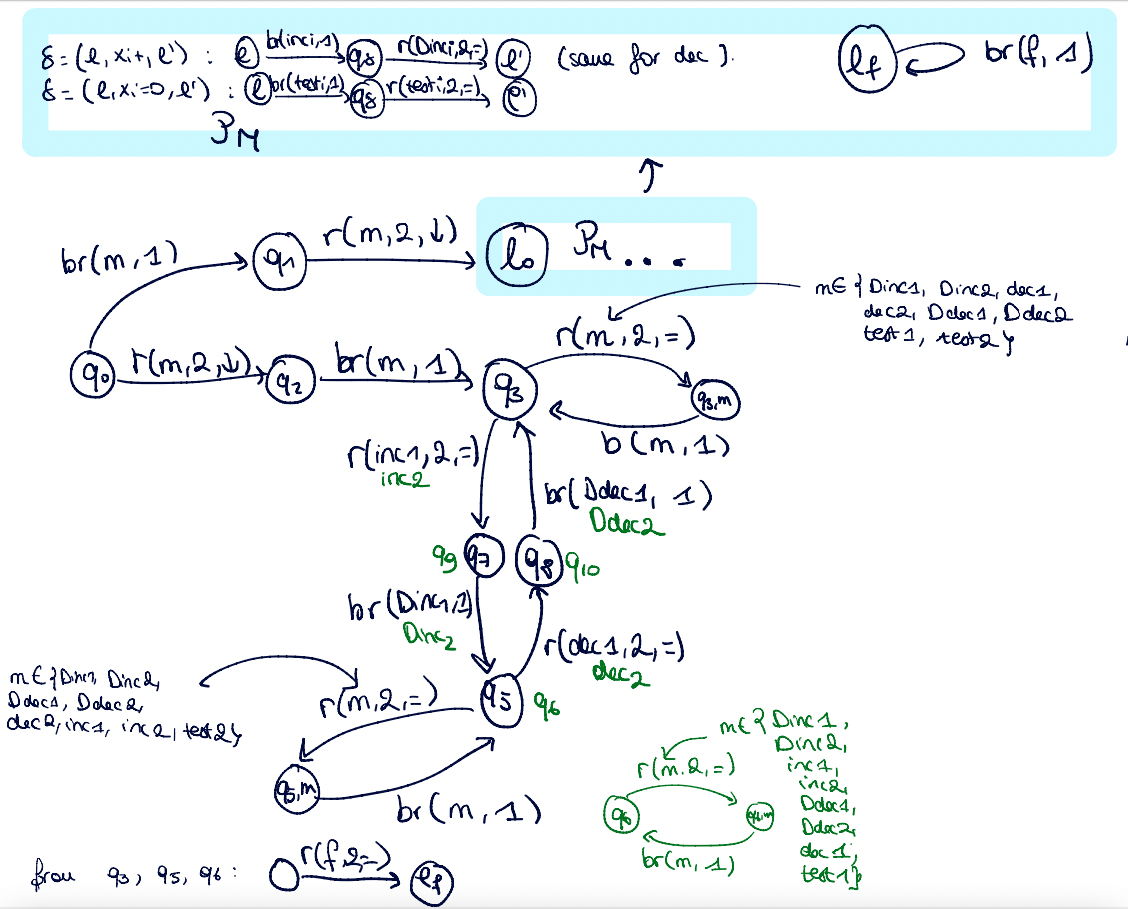
\includegraphics[scale=0.4]{./Figures/construction-target.png}
			\caption{protocol} \label{prot}
		\end{figure}
		
		
		
		\begin{lemma}
			If there exists an initial execution in $M$ ending in $(\ell_f, v_1, v_2)$ for $v_1, v_2 \in \nats$, then there exists a run $\rho = \config_0 \step{*} \config_f$ with $\config_f(a) = q_f$ for all $a \in \agentsof{\rho}$.
		\end{lemma}
		
		\begin{proof}
			\luin{for now there is no intuition in this proof, please feel free to add whatever }
			Assume there is an initial execution $(\ell_0, 0, 0) \stepMM{\delta_1} (\ell_1, v_1^1, v_2^1) \stepMM{\delta_2} \dots \stepMM{\delta_k} (\ell_k, v_1^k, v_2^k)$ such that $\ell_k = \ell_f$, and note $N = \max_{1 \leq i \leq k}(v_1^i + v_2^i)$. Consider an initial configuration of $\prot$ with $N+ 1$ agents $\config_0$. We note $\agents = \{1, \dots, N+1\}$. From this initial configuration, we let the agent 1 takes the transition $(q_0, \br{m}{1}, q_1)$, and we choose this message to be received by the agent 2 only, with the transition $(q_0, \rec{m}{2}{\enregact}, q_2)$. This way, we construct $\config_1$ such that $\config_1(1) = (q_1, \data{\config_0}(1))$, $\st{\config_1}(2) =q_2$, $\data{\config_1}(2,2) = \data{\config_1}(1,1)$ and $\data{\config_1}(2,1) = \data{\config_0}(2,1)$. Note that for all other agents $a$, $\config_1(a) = \config_0(a)$. Now we will construct a sequence of configurations in the following way: for $1 \leq i < N$, from $\config_i$, agent $(i+1)$ takes the transition $(q_2, \br{m}{1}, q_3)$ and agent $(i+2)$ takes the transition $(q_0, \rec{m}{2}{\enregact}, q_2)$. One can prove by induction that $\config_1 \stepMM{} \config_2 \stepMM{} \dots \stepMM{} \config_N$ and that for all $1 \leq i \leq N$, and for all $j \in \agents$:
			\begin{itemize}
				\item if $j = 1$, $\st{\config_i}(j) = q_1$,
				\item if $1 < j \leq i$, $\st{\config_i}(j) = q_3$, and $\data{\config_i}(j,2) = \data{\config_i}(j-1,1)$
				\item if $j = i+1$, $\st{\config_i}(k) = q_2$, and $\data{\config_i}(j,2) = \data{\config_i}(j-1,1)$,
				\item if $j > i+1$, $\st{\config_i}(j) = q_0$.
			\end{itemize}
		\luin{proof by induction here}
		Finally, from $\config_N$ there is a last step before starting to simulate the execution of the machine: agent $(N+1)$ takes the transition $(q_2, \br{m}{1}, q_3)$ and agent 1 the transition $(q_1, \rec{m}{2}{\enregact}, \ell_0)$ reaching the configuration $\config'_{0}$ where $\config'_0$ is such that: $\forall i \in \agents$, if $i = 1$, $\st{\config'_0}(i) = \ell_0$, otherwise, $\st{\config'_0}(i) = q_3$, and $\data{\config'_0}(i, 2) = \data{\config'_0}((i+1)\%(N+1), 1)$. Note that, by construction, for all agent $i,j  \in \agents$ with $i \ne j$, $\data{\config'_0}(i, 1) \ne \data{\config'_0}(j,1)$.
		\luin{here add a figure to illustrate the situation of the agents }
		
		From $\config'_0$, we can start to simulate the execution between $(\ell_0, 0, 0)$ and $(\ell_k, v_1^k , v_2^k )$. We will do so by induction: we shall build a path from $\config'_0$ to $\config'_i$ for $0\leq i\leq k$, where $\config'_i$ is such that:  
		\begin{itemize}
			\item $\st{\config'_i}(1) = \ell_i$,
			\item there exists $x_1, \dots x_{v_1^i} \in \agents$ such that $\st{\config'_i}(x_j) = q_5$ for all $1 \leq j \leq v_1^i$;
			\item there exists $y_1, \dots y_{v_2^i} \in \agents$ such that $\st{\config'_i}(y_j) = q_6$ for all $1 \leq j \leq v_2^i$;
			\item for all $a \in \agents \setminus \{1, x_1, \dots, x_{v_1^i}, y_1, \dots y_{v_2^i}\}$, $\st{\config'_i}(a) = q_3$;
			\item $\data{\config'_i} = \data{\config'_0}$.
		\end{itemize} 
	For $i =0$, the construction is trivial as $\gamma'_0$ satisfies the desired properties.
	
		
	In the rest of this proof keep in mind that for any agent $a \in \agents$, and any configuration $\config$ that we will build, $\data{\config}(a,1) = \data{\config}((a+1)\%(N+1),2)$.\\
	
		\textbf{Construction of $\gamma'_{i+1}$.}
		We assume $\delta_{i+1} = (\ell_i, \inc{x_1}, \ell_{i+1})$, by definition of $N$, we observe that, as a consequence $v_1^i + v_2^i < N$, and so, by induction hypothesis, there exists $a \in \agents$ such that $\st{\config'_i}(a) = q_3$. We note $a_{\mathtt{new}}$ the minimal agent in such a state in $\config'_i$, formally $a_{\mathtt{new}} = \min_{a \in \agents}(\st{\config'_i}(a) = q_3)$. In the following we note $\delta = \delta_{i+1}$. From $\config'_i$, we build the path $\config_{1} \step{} \config_{2} \step{} \dots \step{} \config_{N+1}$, where $\config_{1} = \config'_i$ and for all $2 \leq j \leq N+1$:
		\begin{itemize}
			\item if $j< a_{\mathtt{new}}$, $\st{\config_j}(j) = (q, \mathtt{inc1})$ where $q = \st{\config_{j-1}}(j)$, 
			\item if $j> a_{\mathtt{new}}$, $\st{\config_j}(j) = (q, \mathtt{Dinc1})$ where $q = \st{\config_{j-1}}(j)$,
			\item if $j = a_{\mathtt{new}}$, $\st{\config_j}(j) = q_7$;
			\item for all $2 \leq k < j$, if $k\ne a_{\mathtt{new}}$, $\st{\config_j}(k) = q$ where $q = \st{\config_{1}}(j)$, otherwise $\st{\config_j}(k) = q_5$;
			\item for all $k > j$,  $\st{\config_j}(k) = \st{\config_1}(k)$;
			\item $\st{\config_j}(1) = q_\delta$;
			\item $\data{\config_j}= \data{\config_1}$.
		\end{itemize}
		We will first see how to build $\config_2$ from $\config_1$ and then how to build $\config_{j+1}$ from $\config_j$.
		\begin{itemize}
			\item\textbf{$\config_2$ from $\config_1$:} agent 1 takes the transition $(\ell_i, \br{\mathtt{inc1}}{1}, q_{\delta})$, and (i) if $a_{\mathtt{new}} \ne 2$, agent 2 takes the transition $(q, \rec{\mathtt{inc1}}{2}{=}, (q,\mathtt{inc1}))$ where $q = \st{\config_1}(2)$, (ii) otherwise, agent 2 takes the transition $(q_3, \rec{\mathtt{inc1}}{2}{=}, q_7)$.
			
			\item\textbf{$\config_{j+1}$ from $\config_j$ when $j= a_{\mathtt{new}}$:} the agent $j$ takes the transition $(q_7, \br{\mathtt{Dinc1}}{1}, q_5)$ and the agent $j+1$ takes the transition $(q, \rec{\mathtt{Dinc1}}{2}{=}, (q,\mathtt{Dinc_1}))$ where $q = \st{\config_j}(j+1)$. Note that, as $j = a_{\mathtt{new}}$, $j+1 \not = a_{\mathtt{new}}$.
			
			\item\textbf{$\config_{j+1}$ from $\config_j$ when $j \ne a_{\mathtt{new}}$:} the agent $j$ takes the transition $((q,m), \br{m}{1}, q)$ where $q = \st{\config_1}(j)$, $m \in \{\mathtt{inc1}, \mathtt{Dinc1}\}$ and $(q,m) = \st{\config_{j}}(j)$. If $j+1 \ne a_{\mathtt{new}}$, agent $j+1$ takes the transition $(q, \rec{m}{2}{=}, (q,m))$ if $j+1$ where $q = \st{\config_j}(j+1)$, otherwise it takes the transtion $(q_3, \rec{m}{2}{=}, q_7)$. Note that if $j+1 = a_{\mathtt{new}}$, then $m = \mathtt{inc1}$, $a_{\mathtt{new}}$ is the first agent to send the message $\mathtt{Dinc1}$ in the path.
		\end{itemize}
		Finally, in order to finish the construction of $\config'_{i+1}$, what is left to show is how to go from $\gamma_{N+1}$ to $\gamma'_{i+1}$. We do so in the following way: from $\gamma_{N+1}$ the agent $N+1$ is either on state $q_7$ if $a_{\mathtt{new}} = N+1$, either on a state $(q,\mathtt{Dinc1})$ where $q = \st{\config_1}(N+1)$. From $\gamma_{N+1}$, agent $N+1$ takes either a transition $(q_7, \br{\mathtt{Dinc1}}{1}, q_5)$ if $a_{\mathtt{new}} = N+1$, either a transition $((q,\mathtt{Dinc1}), \br{\mathtt{Dinc1}}{1}, q)$. Hence, agent 1 can take the transition $(q_\delta, \rec{\mathtt{Dinc}}{2}{=}, \ell_{i=1})$ (recall that $\data{\gamma_{N+1}}(1,2) = \data{\gamma_1}(1,2) = \data{\gamma'_0}(1,2) = \data{\gamma'_0}(N+1,1) = \data{\gamma_{N+1}}(N+1,1)$). The reached configuration is $\gamma'_{i+1}$. 
		
		One can verify that the only agent $a \in \agents \setminus \{1\}$ for which $\st{\gamma'_i}(a) \not = \st{\gamma'_{i+1}}(a)$ is $a_{\mathtt{new}}$ and its new state is $q_5$. From this, we conclude that $\gamma'_{i+1}$ satisfies the desired properties.
		%: $\st{\gamma'_{i+1}}(1) = \ell_{i+1}$, there exists $x_1, \dots, x_{v_1^i} , x_{v_1^{i+1}}\in \agents$  ($x_{v_1^{i+1}} = a_{\mathtt{new}}$) such that $\st{\gamma'_{i+1}}(x_j) = q_5$ for all $1 \leq j \leq v_1^i$, 
		
		The proof is done in an analogous way when $\delta_{i+1} = (\ell_i, \dec{\cpt_1}, \ell_{i+1})$ (this time $a_{\mathtt{new}}$ will be the first agent present on the state $q_5$) and of course the same can be done for increments and decrements on $\cpt_2$.
		
		When it comes to test to 0 of the counter $\cpt_1$, the transmitted message will be the same during all the path between $\gamma'_i$ and $\gamma'_{i+1}$. As by induction hypothesis, all agents are either on state $q_3$ or $q_6$, every agent will be able to receive and broadcast the message $\mathtt{test1}$. \lu{est ce que l'on veut écrire formellement ce cas là également ?}\\
		
		\luin{end of the proof}
		
		Now that we have build the path $\gamma'_0 \step{*} \gamma'_k$, it is easy to complete the execution to reach a configuration in wich all agents have local state $\ell_f$. Indeed, by construction $\st{\gamma'_k}(1) = \ell_f$. Hence, agent 1 can broadcast the message $\mathtt{f}$, received by agent 2, agent 2 then reaches $\ell_f$, and so on until all agents are on state $\ell_f$.\lu{more formal?} 
		\end{proof}
		
		\begin{lemma}
			If there exists a run $\rho = \config_0 \step{*} \config_f$ with $\config_f(a) = q_f$ for all $\agentsof{\rho}$, then there exists an initial execution in $M$ ending in $(\ell_f, v_1, v_2)$ for $v_1, v_2 \in \nats$.
		\end{lemma}
		

	\end{proof}
\end{document}